% Chapter Template

\chapter{Experiments} % Main chapter title

\label{Chapter3} % Change X to a consecutive number; for referencing this chapter elsewhere, use \ref{ChapterX}

\lhead{Chapter 3. \emph{Experiments}} % Change X to a consecutive number; this is for the header on each page - perhaps a shortened title

%----------------------------------------------------------------------------------------
%	SECTION 1
%----------------------------------------------------------------------------------------

\section{Experimental Setup}

Data Center networks often use a fat-tree topology as this topology is easy to maintain
and to scale. To simulate a fat-tree topology as seen in data center networks, 4 physical servers and 2 data plane programmable switches were used. Each switch
was virtualized to create 5 switches using 10G loopback links. So, we have 10 switches in total, with 4 of them as top-of-rack or edge switches,
4 of them as aggregate switches, and 2 as core switches (Figure \ref{fig:Topology})

\begin{figure}[htbp]
	\centering
		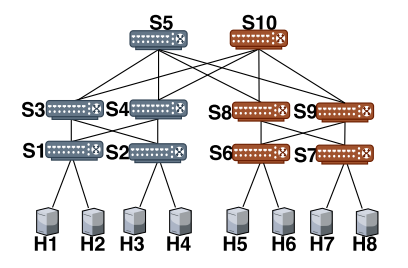
\includegraphics{Figures/Topology.png}
		\rule{35em}{0.5pt}
	\caption[Evaluation Topology]{Evaluation Topology}
	\label{fig:Topology}
\end{figure}

% The rest of this chapter is structured as follows: For a potential fault that can occur in the network, we have
% \begin{itemize}
%     \item A section on the description of the fault
%     \item A section on the configuration of switches and hosts for reproducing the fault
%     \item A section on how the proposed fault can be diagnosed using SQL queries
% \end{itemize}

% The last section presents a unified scheme for diagnosing faults in networks that has been built on logic that was developed
% in preceding sections.

\section{SQL Database Schema}

The relational schema for the packet records collected from switches is as shown in Figure \ref{fig:Schema}
\begin{figure}[htbp]
	\centering
		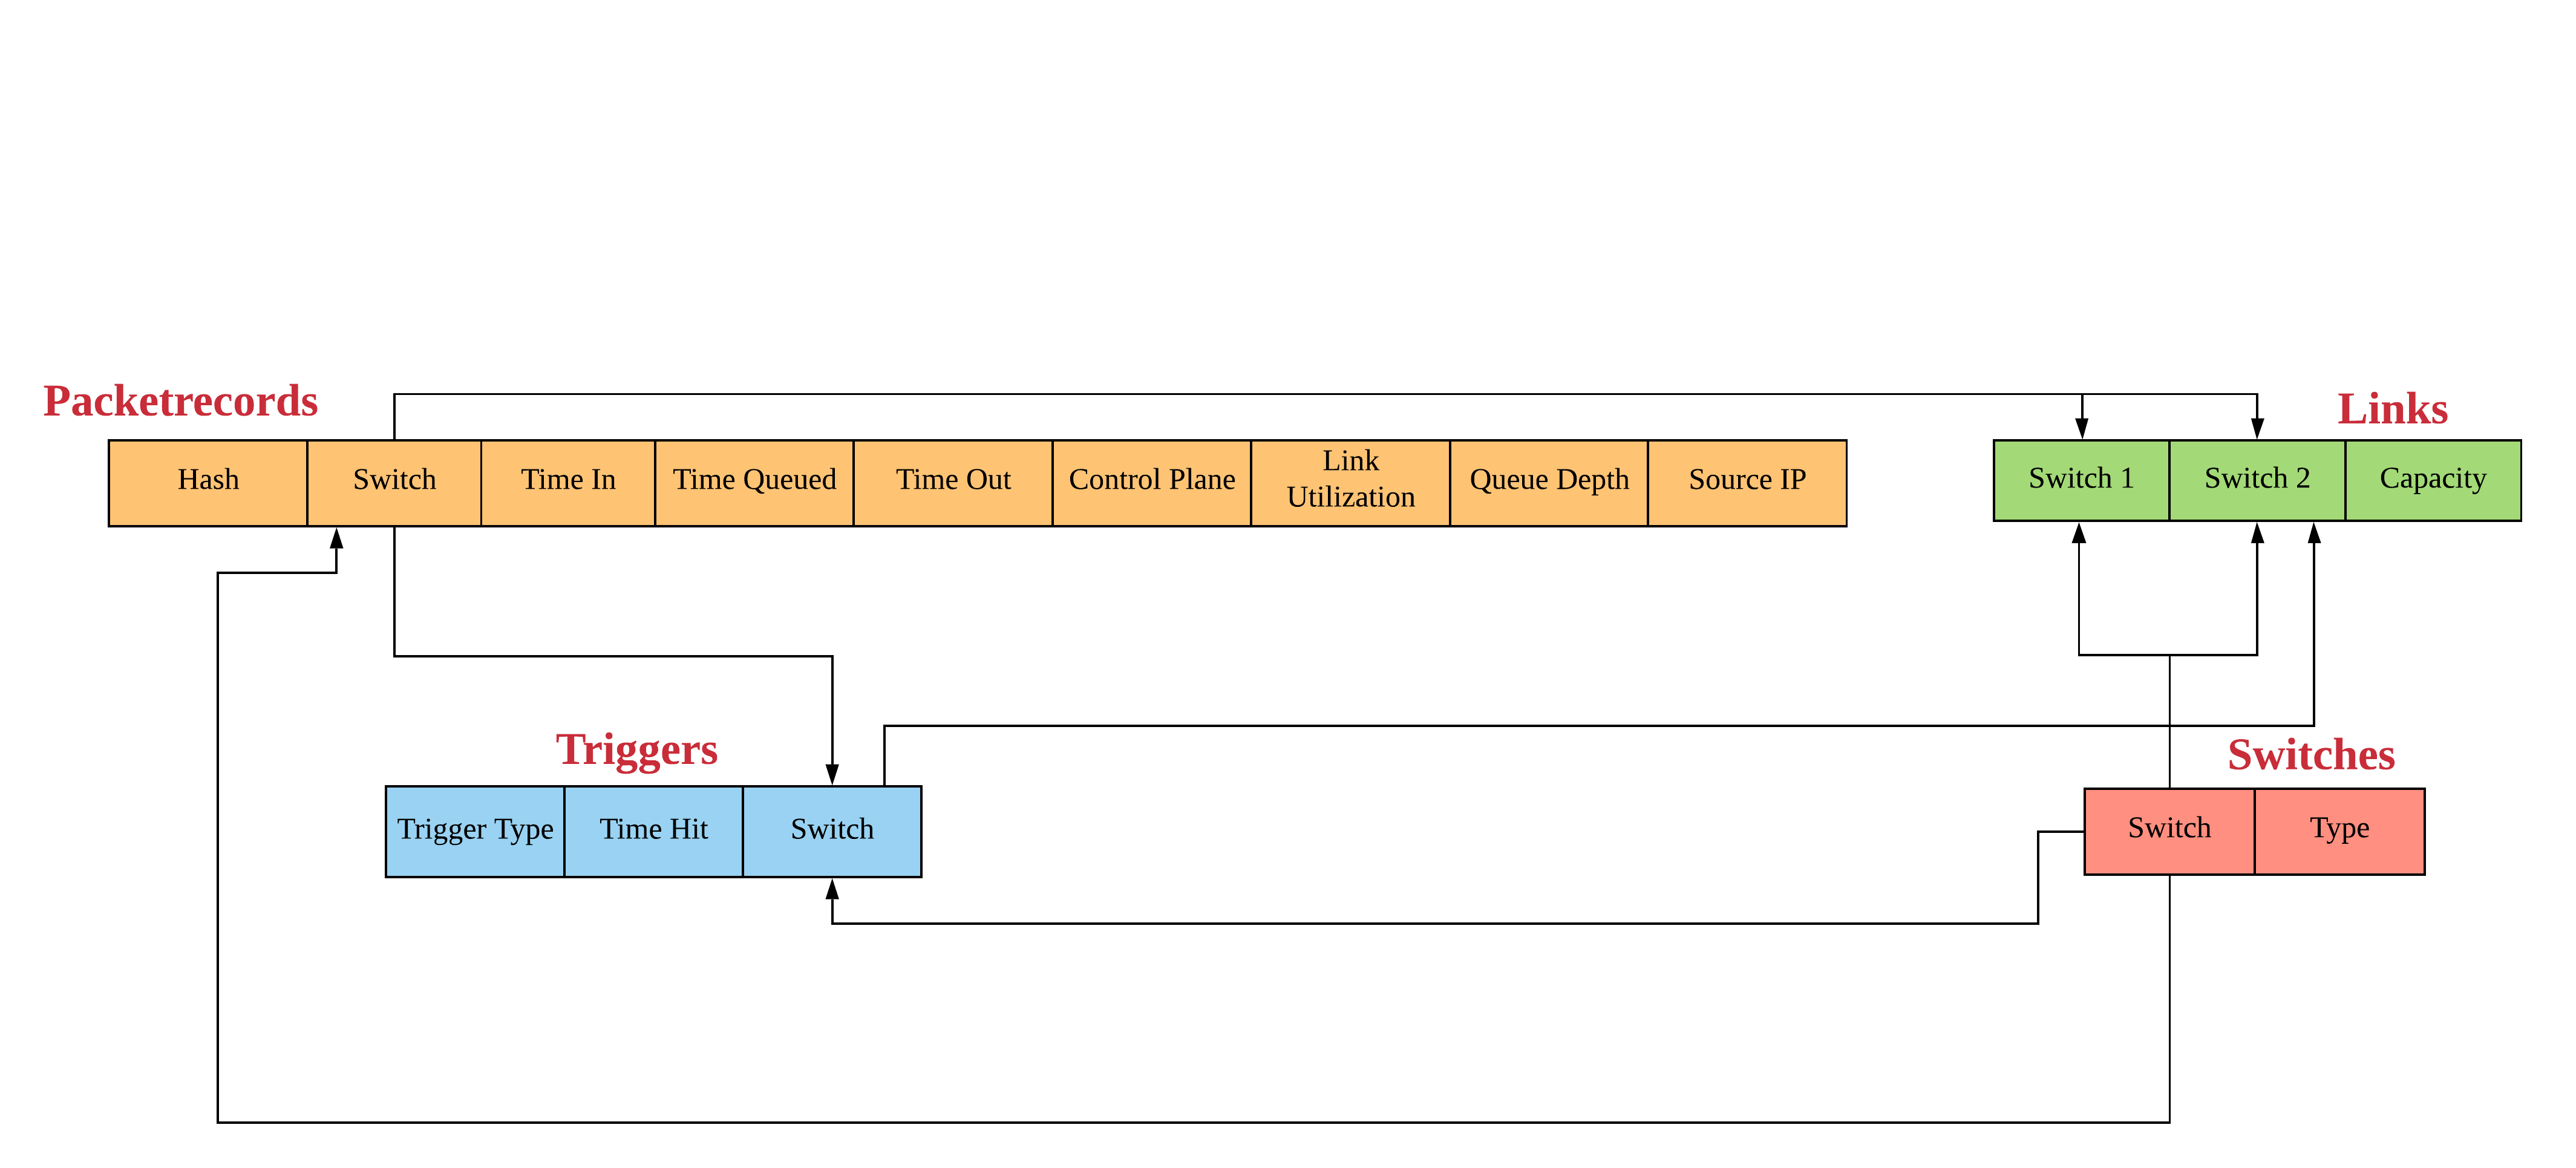
\includegraphics[width=1.0\columnwidth]{Figures/Schema.png}
		\rule{35em}{0.5pt}
	\caption[RDBMS Schema]{Database Schema}
	\label{fig:Schema}
\end{figure}

\subsection{The Switches table}

This table stores two columns described below:
\begin{itemize}
	\item Switch - The identifier of the switch, a string ID that is used to uniquely
	identify each switch
	\item Type - This column specifies the type of the switch. For the purpose of our 
	demonstrations, Switch type could either be a ToR switch (top of rack) or a non-ToR switch.
\end{itemize}

\subsection{The Triggers table}

This table stores three columns described below:
\begin{itemize}
	\item Trigger Type - an identifier for the type of trigger, which can indicate what was
	the cause of the fault in the network. As an example, the switch might be configured to 
	create a trigger when the queue depth at a switch exceeds a certain number.
	\item Time Hit - the time at which the trigger condition was raised, 
	in the format of a 64 bit representation. The most significant bit in the decimal representation of the 64
	bit number would denote the number of seconds passed, while the remaining digits would denote the precision in nanoseconds.
	For example, the number 1435756194 (stored as a 64 bit number) would mean 1.435756194 seconds.
	\item Switch - the identifier of the switch that raised the trigger.
\end{itemize}

\subsection{The Links table}

This table stores three columns described below:
\begin{itemize}
	\item Switch 1 - the identifier of the source switch for the link.
	\item Switch 2 - the identifier of the destination switch for the link.
	\item Capacity - the link capacity in Gbps.
\end{itemize}

\subsection{The Packetrecords table}

This table stores the following 9 columns corresponding to each packet,
as described below. There exists such a tuple for every packet that leaves any switch in the network.
\begin{itemize}
	\item Hash - the hash of a packet, to identify it uniquely
	\item Switch - the identifier of the switch the packet has just left.
	\item Time In - the time at which the packet enters the switch, in nanosecond precision.
	\item Time Queued - the duration for which the packet is queued in the switch.
	\item Time Out - the time at which the packet leaves the switch, in nanosecond precision.
	\item Control Plane - an identifier for the version of control plane that is presently running in the switches.
	\item Link Utilization - the current egress link utilization of the switch, as measured in the data plane of the switch itself.
	This field is later used to corroborate our calculations for egress throughput.
	\item Queue Depth - the current length of the queue in the switch.
	\item Source IP - the source IP of the packet that the 9-tuple represents.
\end{itemize}